\documentclass[10pt]{beamer}
\usetheme{Madrid}

\usepackage[utf8]{inputenc}
\usepackage[T1]{fontenc}
\usepackage{amsmath}
\usepackage{amsfonts}
\usepackage{amssymb}
\usepackage{graphicx}
\usepackage{float}
\usepackage{array}
\usepackage{placeins}
\renewcommand{\figurename}{Figura}
\renewcommand\tablename{Tabla}

\author{Czarnievicz, Pereda, Pereira}
\title []{¿Es cara la nafta en Uruguay?}
\subtitle []{Competencia en el mercado de combustibles líquidos en Uruguay}

\date{}
\institute []{Organización Industrial, FCEA - UdelaR}

\begin{document}
\maketitle
\begin{frame}
\tableofcontents
\end{frame}

%%%%%%%%%%%%%%%%%%%%%%%%%%%%%%%
%%%% OBJETIVOS DEL TRABAJO %%%%
%%%%%%%%%%%%%%%%%%%%%%%%%%%%%%%

\section{Objetivos del trabajo}

\begin{frame}{Objetivos del trabajo}

Aportar elementos para una discusión más rigurosa sobre si mejorar la regulación actual del sistema de bonificaciones que perciben las estaciones de servicio o, alternativamente, proponer un sistema que se aproxime a la liberalización del precio final.

\end{frame}

%%%%%%%%%%%%%%%%%%%%%%%%%%%%%%%%%
%%%% DESCRIPCIÓN DEL MERCADO %%%%
%%%%%%%%%%%%%%%%%%%%%%%%%%%%%%%%%

\section{Descripción del mercado}

\begin{frame}[allowframebreaks]{Descripción del mercado}

\begin{itemize}
\item Oferta
	\begin{itemize}
	\item ANCAP: monopolio importador y refinador de petróleo.
	\item Distribuidoras: transportan los productos desde ANCAP hacia las estaciones mediante la contratación de fletes.
		\begin{itemize}
		\item DUCSA 
		\item Petrobras
		\item AXION
		\end{itemize}
	\item Estaciones de servicio (EESS): encargadas de realizar la venta al público, operadas por empresas privadas bajo el sello de la distribuidora correspondiente. Pueden ser dueñas o no de la propiedad en la cual opera la estación.
	\end{itemize}
\end{itemize}

\begin{itemize}
\item Demanda
	\begin{itemize}
	\item Familias y hogares
	\item Firmas
	\item Aeropuertos 
	\end{itemize}
\end{itemize}

\framebreak

\begin{itemize}
\item Regulador
	\begin{itemize}
	\item \underline{ANCAP}: fija el máximo precio intermedio y el máximo precio final del combustible. Decretado por el Poder Ejecutivo ante sugerencia del directorio de ANCAP.
	\item \underline{URSEA}: fiscaliza y controla la calidad de los combustibles a lo largo de toda la cadena. Realiza estudios comparativos para saber si los valores fijados por ANCAP están en consonancia con los valores que las gasolinas tendrían si se las importara. 
	\end{itemize}
\end{itemize}
\end{frame}

\begin{frame}{Dinámica del mercado de combustibles líquidos}

\begin{center}
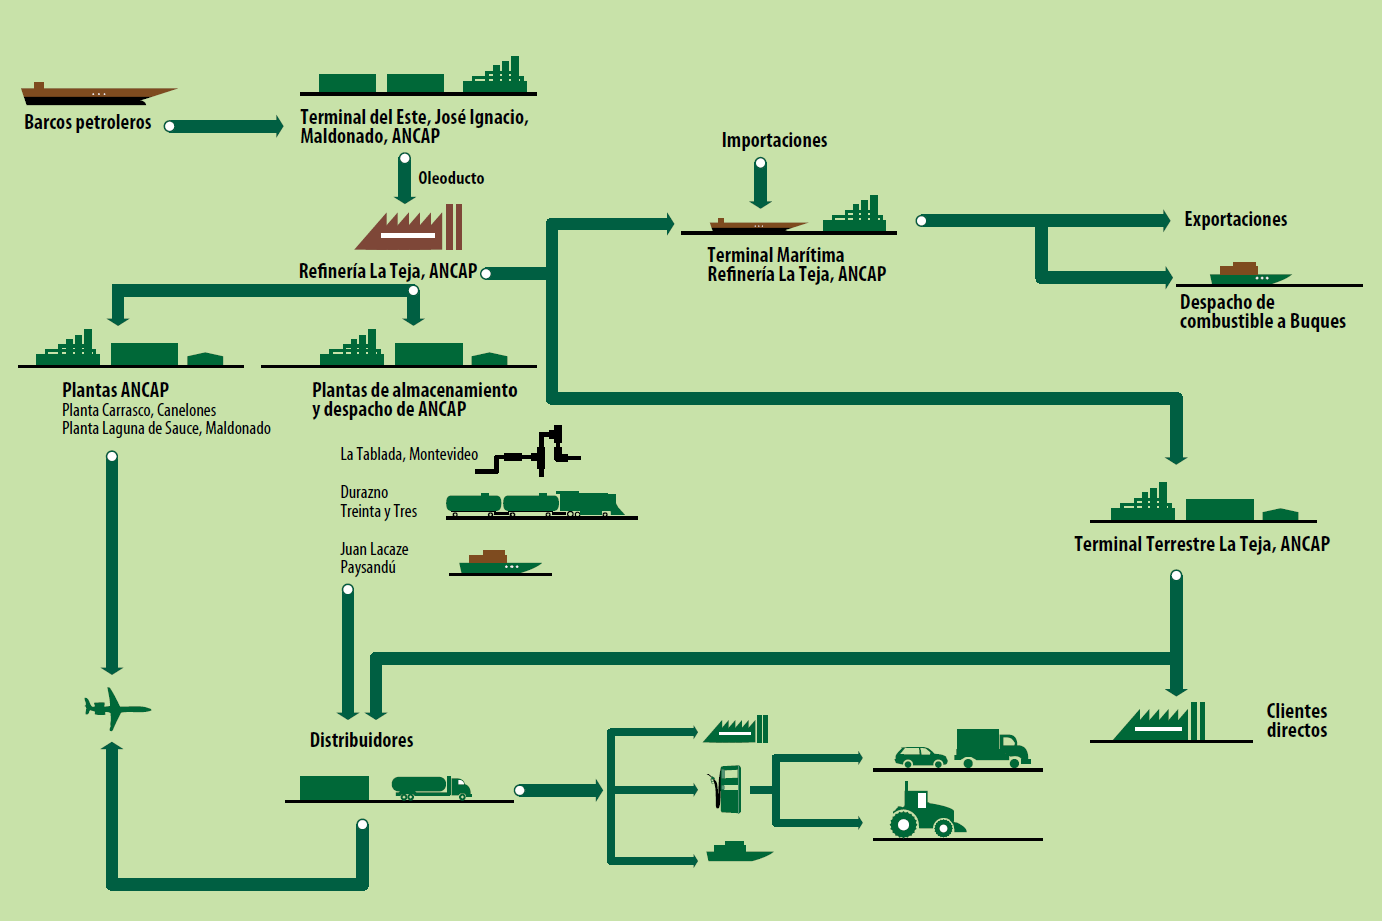
\includegraphics[scale=0.25]{imagen2.png}
\end{center}
\FloatBarrier
\noindent\textbf{Fuente:} Anuario 2011-2012 de la Unidad Reguladora de Servicios de Energía y Agua (URSEA).

\end{frame}

\begin{frame}[allowframebreaks]{Composición del mercado de distribución}

\begin{center}
Cantidad de estaciones de servicio y distribución según proveedora \\
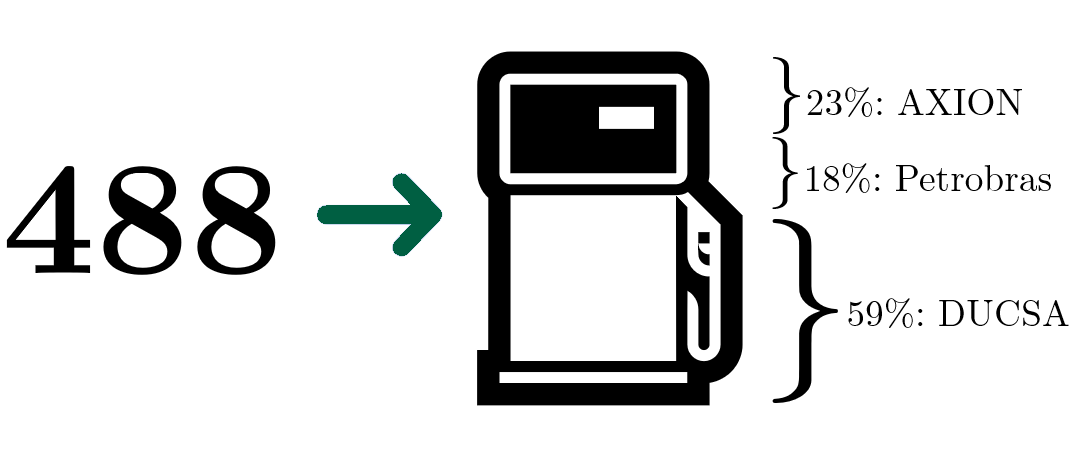
\includegraphics[scale=0.4]{imag1.png}
\end{center}

\framebreak

\begin{center}
Mapa de ubicación de las estaciones de servicio en el territorio nacional según la distribuidora \\
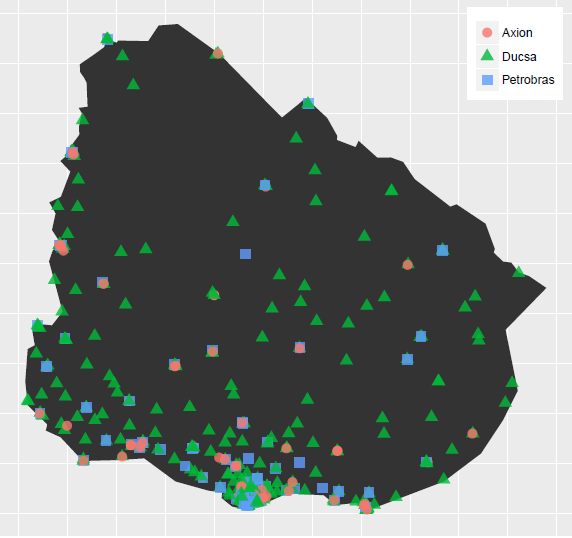
\includegraphics[scale=0.5]{mapaeess.png}
\end{center}
\FloatBarrier
\noindent\textbf{Fuente:} elaboración propia en base a datos de la Unidad Reguladora de Servicios de Energía y Agua (URSEA).

\framebreak

\begin{center}
Mapa de ubicación de las estaciones de servicio en Montevideo y el área metropolitana según la distribuidora \\
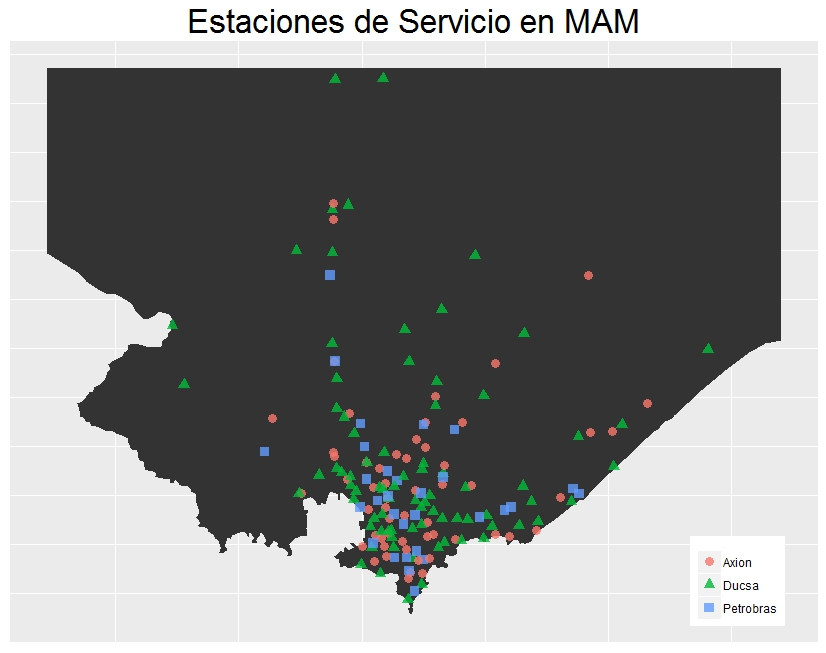
\includegraphics[scale=0.35]{mapaeessmam.png}
\end{center}
\FloatBarrier
\noindent\textbf{Fuente:} elaboración propia en base a datos de la Unidad Reguladora de Servicios de Energía y Agua (URSEA).

\end{frame}

%%%%%%%%%%%%%%%%%%%%%
%%%% PARAMÉTRICA %%%%
%%%%%%%%%%%%%%%%%%%%%

\begin{frame}[allowframebreaks]{Paramétrica}

La bonificación puede ser representada, según CPA FERRERE (2016), por la siguiente ecuación:
$$ B_1=B_0\ldotp \frac{Vt_0\ldotp f(x)}{Vt_1 \ldotp Ct_0} $$

siendo $f(x) = \frac{IPC_t}{IPC_0}\times 458616.2 + \frac{SP_t}{SP_0}\times310736.8 + \frac{URA_t}{URA_0}\times 209952.4 + \frac{USD_t}{USD_0}\times 9531.3 + \frac{Pnafta_t}{Pnafta_0}\times 41484.3$

\begin{itemize}
\item Reconoce los siguientes componentes:
	\begin{itemize}
	\item Variación de precios (mediante el IPC)
	\item Salario de los pisteros
	\item Alquiler del predio
	\item Variación del tipo de cambio
	\item Precio de la gasolina súper 95
	\item Volumen de litros vendidos por la estación promedio
	\item Costos totales de la estación "tipo"
	\end{itemize}
\end{itemize}

\begin{itemize}
\item Desde mediados del 2016, se encuentra congelada. Se acordó entre la UNVENU y ANCAP futuras actualizaciones trimestrales mediante el IPC y el IMS del valor congelado.
\end{itemize}

\framebreak

\begin{center}
Composición del precio de un litro de Súper y Gasoil a abril de 2017 (en pesos uruguayos) \\
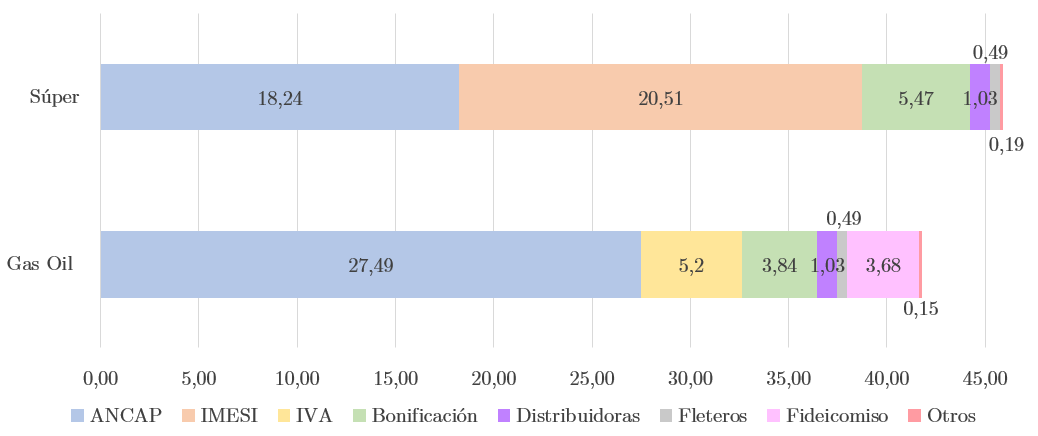
\includegraphics[scale=0.5]{descom.png} 
\end{center}
\FloatBarrier
\noindent\textbf{Fuente:} elaboración propia en base a datos de la Unidad Reguladora de Servicios de Energía y Agua (URSEA).

\end{frame}

%%%%%%%%%%%%%%%%%%%
%%%% HIPÓTESIS %%%%
%%%%%%%%%%%%%%%%%%%

\section{Hipótesis}

\begin{frame}{Hipótesis}
\begin{itemize}
\item Existe margen de mejora en términos de eficiencia:
	\begin{itemize}
	\item La parámetrica no reconoce la heterogeneidad en la estructura de costos de las EESS.
	%Cantidad de pisteros, con/sin camión repartidor, ubicación geográfica, alquiler predio, tamaño estación
	\item La liberalización del precio final del combustible ha de estar condicionada a la densidad poblacional y a las características particulares de cada firma.
	\end{itemize}
\item Se debe fortalecer la capacidad de contralor del regulador.
\end{itemize}

%\begin{center}
%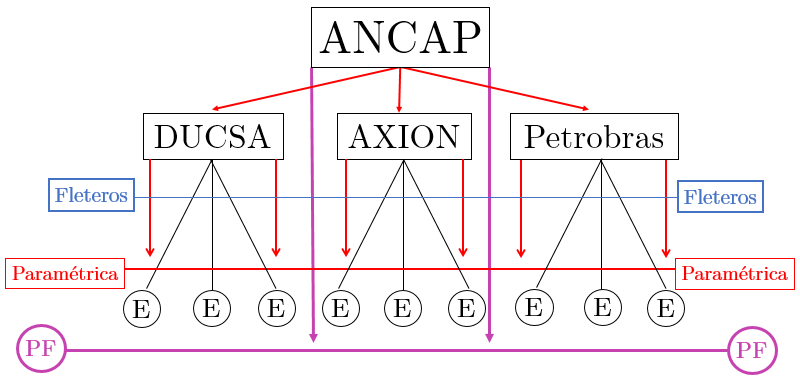
\includegraphics[scale=0.5]{cadenaeess.png} 
%\end{center}

\end{frame}

%%%%%%%%%%%%%%%%%%%%%%%%%%%%%%%%%%%%%%%%%%%%%%%%%%
%%%% GANADORES Y PERDEDORES DE LA PARAMÉTRICA %%%%
%%%%%%%%%%%%%%%%%%%%%%%%%%%%%%%%%%%%%%%%%%%%%%%%%%

\begin{frame}{¿Quiénes ganan y quiénes pierden con la paramétrica?}

\begin{center}
\begin{tabular}{| >{\centering\arraybackslash} m{5cm} | >{\centering\arraybackslash} m{5cm} |}
	\hline
	\textbf{Ganadores} & \textbf{Perdedores} \\
	\hline
	EESS con camiones & EESS sin camiones \\
	\hline
	Grandes superficies & Medianas y pequeñas superficies \\
	\hline
	Quienes no pagan alquiler & - \\
	\hline
	Quienes no cobran la mayor parte de sus ventas a través de medios electrónicos de pago & Quienes cobran la mayor parte de sus ventas a través de medios electrónicos de pago \\
	\hline
\end{tabular}
\end{center}

\end{frame}

%%%%%%%%%%%%%%%%%%%%%%%%%%%%%%%%%%%%
%%%% PROS & CONS DE LIBERALIZAR %%%%
%%%%%%%%%%%%%%%%%%%%%%%%%%%%%%%%%%%%

\section{Pros y cons de liberalizar el precio}

\begin{frame}{Pros y cons de liberalizar el precio}

\begin{itemize}
\item Liberalizar el precio final no necesariamente implica una baja en el mismo, debido a que:
	\begin{itemize}
	\item Los mayores determinantes del precio son los impuestos y el precio al que ANCAP vende el combustible
	\item ANCAP es un monopolio público que enfrenta los siguiente problemas:
		\begin{enumerate}
		\item No tiene incentivos a ser eficiente
		\item Múltiples principales
		\item Gobernanza sujeta al ciclo político
		\end{enumerate} 
	\item Posible colusión en áreas con pocas estaciones (necesidad de un regulador fuerte)
	\item URSEA desarticulado en su potestad de regulador económico
	\end{itemize}
\item A priori no podríamos señalar los pros y cons dado que debe establecerse un modelo formal estimable para cuantificarlos.
\item Lo único esperable es que las EESS más pequeñas cierren. Se debe considerar entonces la pérdida de empleos en esta rama así como también en sus mercados conexos.
\end{itemize}

\end{frame}

%%%%%%%%%%%%%%%%%%%%%%%%%%%%%%%%
%%%% CAPACIDAD DE CONTRALOR %%%%
%%%%%%%%%%%%%%%%%%%%%%%%%%%%%%%%

\section{Capacidad de contralor}
\begin{frame}{Capacidad de contralor}
\begin{itemize}
\item Las empresas públicas requieren de un regulador para inducir un comportamiento eficiente dado que, tienen que atender a un cúmulo de objetivos económicos y políticos, muchos de ellos contrapuestos (Domingo, Zipitría, 2015).
\item Si bien en Uruguay existe un organismo regulador, la URSEA, desde 2011 se le quitó su potestad de contralor económico manteniéndole únicamente su capacidad de control de calidad y control técnico (Domingo, Ponce, Zipitría, 2016).
\item Los directores de la URSEA son designados por el Poder Ejecutivo, con cargos de 6 años. Adicionalmente, el Presidente de la República tiene capacidad derogativa sobre sus fallos (Domingo, Ponce, Zipitría, 2016). 
\end{itemize}
\end{frame}

\section{Reflexiones preliminares}

\begin{frame}{Reflexiones preliminares}
\begin{itemize}
\item Hasta el momento no es claro que haya una ganancia de eficiencia con la liberalización del precio final del combustible, en contraposición con una reformulación de la paramétrica.
\item Independientemente de qué sistema sea el que se implemente, es menester fortalecer el rol del regulador para procurar el funcionamiento óptimo del mercado.
\item En la misma línea con lo anterior, es necesario establecerle objetivos y metas claras a ANCAP.
\end{itemize}
\end{frame}

\end{document}